\documentclass{article}[18pt]
\ProvidesPackage{format}
%Page setup
\usepackage[utf8]{inputenc}
\usepackage[margin=0.7in]{geometry}
\usepackage{parselines} 
\usepackage[english]{babel}
\usepackage{fancyhdr}
\usepackage{titlesec}
\hyphenpenalty=10000

\pagestyle{fancy}
\fancyhf{}
\rhead{Sam Robbins}
\rfoot{Page \thepage}

%Characters
\usepackage{amsmath}
\usepackage{amssymb}
\usepackage{gensymb}
\newcommand{\R}{\mathbb{R}}

%Diagrams
\usepackage{pgfplots}
\usepackage{graphicx}
\usepackage{tabularx}
\usepackage{relsize}
\pgfplotsset{width=10cm,compat=1.9}
\usepackage{float}

%Length Setting
\titlespacing\section{0pt}{14pt plus 4pt minus 2pt}{0pt plus 2pt minus 2pt}
\newlength\tindent
\setlength{\tindent}{\parindent}
\setlength{\parindent}{0pt}
\renewcommand{\indent}{\hspace*{\tindent}}

%Programming Font
\usepackage{courier}
\usepackage{listings}
\usepackage{pxfonts}

%Lists
\usepackage{enumerate}
\usepackage{enumitem}

% Networks Macro
\usepackage{tikz}


% Commands for files converted using pandoc
\providecommand{\tightlist}{%
	\setlength{\itemsep}{0pt}\setlength{\parskip}{0pt}}
\usepackage{hyperref}

% Get nice commands for floor and ceil
\usepackage{mathtools}
\DeclarePairedDelimiter{\ceil}{\lceil}{\rceil}
\DeclarePairedDelimiter{\floor}{\lfloor}{\rfloor}

% Allow itemize to go up to 20 levels deep (just change the number if you need more you madman)
\usepackage{enumitem}
\setlistdepth{20}
\renewlist{itemize}{itemize}{20}

% initially, use dots for all levels
\setlist[itemize]{label=$\cdot$}

% customize the first 3 levels
\setlist[itemize,1]{label=\textbullet}
\setlist[itemize,2]{label=--}
\setlist[itemize,3]{label=*}

% Definition and Important Stuff
% Important stuff
\usepackage[framemethod=TikZ]{mdframed}

\newcounter{theo}[section]\setcounter{theo}{0}
\renewcommand{\thetheo}{\arabic{section}.\arabic{theo}}
\newenvironment{important}[1][]{%
	\refstepcounter{theo}%
	\ifstrempty{#1}%
	{\mdfsetup{%
			frametitle={%
				\tikz[baseline=(current bounding box.east),outer sep=0pt]
				\node[anchor=east,rectangle,fill=red!50]
				{\strut Important};}}
	}%
	{\mdfsetup{%
			frametitle={%
				\tikz[baseline=(current bounding box.east),outer sep=0pt]
				\node[anchor=east,rectangle,fill=red!50]
				{\strut Important:~#1};}}%
	}%
	\mdfsetup{innertopmargin=10pt,linecolor=red!50,%
		linewidth=2pt,topline=true,%
		frametitleaboveskip=\dimexpr-\ht\strutbox\relax
	}
	\begin{mdframed}[]\relax%
		\centering
		}{\end{mdframed}}



\newcounter{lem}[section]\setcounter{lem}{0}
\renewcommand{\thelem}{\arabic{section}.\arabic{lem}}
\newenvironment{defin}[1][]{%
	\refstepcounter{lem}%
	\ifstrempty{#1}%
	{\mdfsetup{%
			frametitle={%
				\tikz[baseline=(current bounding box.east),outer sep=0pt]
				\node[anchor=east,rectangle,fill=blue!20]
				{\strut Definition};}}
	}%
	{\mdfsetup{%
			frametitle={%
				\tikz[baseline=(current bounding box.east),outer sep=0pt]
				\node[anchor=east,rectangle,fill=blue!20]
				{\strut Definition:~#1};}}%
	}%
	\mdfsetup{innertopmargin=10pt,linecolor=blue!20,%
		linewidth=2pt,topline=true,%
		frametitleaboveskip=\dimexpr-\ht\strutbox\relax
	}
	\begin{mdframed}[]\relax%
		\centering
		}{\end{mdframed}}
\lhead{Software Methodologies - AI Search}


\begin{document}
\begin{center}
\underline{\huge Heuristics}
\end{center}
\section{Heuristics for TSP}
Some heuristics for A* search on the TSP (when formulated so that a state z is a partial tour)\\
\\
h(z)=
\begin{itemize}
	\item Distance to the nearest unvisited city (from the current end-city)
	\item Shortest path of length k through unvisited cities(from the current end-city)
	\item Distance of the "greedy completion" (from the current end-city)
	\item Distance of any "partial" completion, only through k unvisited cities (from the current end city and back to the start)
	\item Distance of the partial tour formed by "inserting" an unvisited city somewhere into the current partial tour
	\item Distance of the partial tour formed by "inserting" a path of k unvisited cities somwehere into the partial tour
	\item ...
\end{itemize}
\section{Heuristic functions for the 8-Puzzle Problem}
We shall investigate heuristic functions through the 8-Puzzle Problem
\begin{itemize}
	\item A matrix of 9 cells, 8 of which contain tiles named 1,2,...,8
	\item Have to move the tiles horizontally and vertically utilising the empty cell
	\item So that the tiles should end up in a specific configuration
\end{itemize}
A particular start state and goal state is shown below:
\begin{center}
	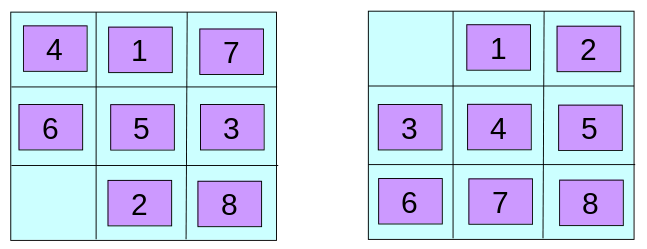
\includegraphics[scale=0.7]{8-puzzle}
\end{center}
\subsection{Common Heuristics}
\begin{itemize}
	\item $h_1(x)$ = the number of misplaced tiles in the corresponding state
	\begin{itemize}
		\item So if z is a node of the search tree whose corresponding state is configuration shown then $h_1(z)$=6
	\end{itemize}
	\item $h_2(x)$ = the sum of the distanced of the tiles from their goal positions where the distance is the Manhattan distance
	\begin{itemize}
		\item i.e., the sum of the horizontal and vertical distanced
		\item So if z is a node of the search tree whose corresponding state is the configuration shown then
	\end{itemize}
	$$h_2(x)=0+3+2+2+1+1+3+0=12$$
\end{itemize}
Both heuristics are admissible\\
Experimental evidence suggests that $h_2$ is better than $h_1$
\subsubsection{Domination}
In fact, $h_2$ is always better than $h_1$\\
\\
Notice that for every node z, $h_2(z)\geqslant h_1(z)$
\begin{itemize}
	\item In general, whenever this is true we say that $h_2$ dominates $h_1$
\end{itemize}
\textbf{Theorem 5}\\
If:
\begin{itemize}
	\item h is admissible
	\item there is a fixed $\epsilon>0$ such that all step-costs exceed $\epsilon$
	\item The branching factor is bounded by b
\end{itemize}
the  A* search necessarily expands all nodes z for which $f(z)<c*$, where $c*$ is the optimal path-cost to a goal node\\
\\
Equivalent to "all nodes z for which $g(z)<c*-h(z)$"\\
\\
But if $h_2(z)\geqslant h_1(z)$ and $g(z)<c*-h_2(z)$ then $g(z)<c*-h_1(z)$
\begin{itemize}
	\item so, any node expanded with heuristic $h_2$ will also be expanded with heuristic $h_1$
	\item moreover, A* search with $h_1$ might expand other nodes too
\end{itemize}
Thus, it is always best to use a heuristic function with higher values, provided it is admissible and efficiently computable
\section{Inventing heuristic functions}
How do these heuristics arise?\\
\\
Whilst $h_1$ and $h_2$ are estimates of remaining path length, they are also accurate estimates for simplified versions of the problem
\begin{itemize}
	\item Suppose that there rules of the problem were changed so that a tile could move to any location and not just to an adjacent vacant cell
	\item Then $h_1$ would be the optimal number of steps to a goal node
	\item Suppose that the rules of the problem were changed so that a file could move one cell up, down, left or right, regardless as to whether the adjacent cell were vacant
	\item Then $h_2$ would be the optimal number of steps to a goal node
\end{itemize}
\begin{defin}[Relaxed problem]
A problem with fewer restrictions on the actions
\end{defin}
Any rule in the original problem should be a rule in the relaxed problem but not necessarily vice versa\\
\\
The cost of an optimal solution in the relaxed problem is an admissible heuristic for the original problem
\begin{itemize}
	\item Any solution for the original problem is a solution for the relaxed problem
\end{itemize}
\subsection{Sub-problem heuristics}
Heuristics can also be derived from the solution-cost of a sub-problem\\
\\
Consider the 8-puzzle problem where the cost is defined as just getting tiles 1,2,3 and 4 to their correct positions (without worrying about the other tiles)\\
\\
The cost of an optimal solution to this sub-problem is used as a heuristic for the main problem
\begin{itemize}
	\item it is necessarily less than the cost of an optimal solution to the original -problem and so the resulting heuristic is admissible
\end{itemize}
However, a relaxed problem or a sub-problem cannot be so difficult to solve that the time taken to compute the heuristic values is excessive
\section{Automatic heuristic derivation}
If a problem is written in a formal language then one can often automatically derive relaxed problems\\
\\
For example, if the 8-Puzzle Problem actions are defined via
\begin{itemize}
	\item a tile can move from cell A to cell B if
	\begin{itemize}
		\item cell A is horizontally or vertically adjacent to cell B and cell B is blank
	\end{itemize}
	then we can generate 3 related problems by removing one or both of the conditions in the conjunction 
\end{itemize}
In order for such heuristics to be practically usable the relaxed problems must be efficiently solvable
\section{More than one heuristic}
When one generates new heuristic functions, one often fails to obtain a heuristic that is clearly the best from those generated
\begin{itemize}
	\item i.e., no function dominates any other function
\end{itemize}
However, one can compose a new heuristic function using all the heuristic functions generated to obtain a dominating heuristic function\\
\\
Suppose $h_1, h_2,..., h_m$ are admissible (resp. consistent) heuristic functions\\
\\
Then the heuristic function h defined via
$$h(x)=\max\{h_1(x),h_2(x),...,h_m(x)\}$$
is admissible (resp. consistent) and dominates each of $h_1,h_2,...,h_m$\\
\\
There is a cost to h
\begin{itemize}
	\item in order to compute h(x), one needs to compute each of $h_1(x),h_2(x),...,h_m(x)$
\end{itemize}
\end{document}